\documentclass{beamer}
\usepackage{relsize}
\usepackage{color}

\usepackage{listings}
\usetheme{CambridgeUS}
%\usepackage{beamerthemesplit} % new 
\usepackage{enumitem}
\usepackage{amsmath}                    % See geometry.pdf to learn the layout options. 
\usepackage{amsthm}                   % See geometry.pdf to learn the layout options. There 
\usepackage{amssymb}                    % See geometry.pdf to learn the layout options. 
\usepackage[utf8]{inputenc} 
\usepackage{graphicx}
\usepackage[english,bulgarian]{babel}
\usepackage[framemethod=tikz]{mdframed}
\usepackage{caption}
\usepackage{tikz}
\usepackage{forest}
\usetikzlibrary{shapes,arrows,positioning,calc,chains}

\lstset{language=C++,
                basicstyle=\ttfamily,
                keywordstyle=\color{blue}\ttfamily,
                stringstyle=\color{red}\ttfamily,
                commentstyle=\color{green}\ttfamily,
                morecomment=[l][\color{magenta}]{\#}
}

\newtheorem{mydef}{Дефиниция}[section]
\newtheorem{lem}{Лема}[section]
\newtheorem{thm}{Твърдение}[section]

\DeclareMathOperator{\restrict}{\upharpoonright}

\setitemize{label=\usebeamerfont*{itemize item}%
  \usebeamercolor[fg]{itemize item}
  \usebeamertemplate{itemize item}}

\setbeamercovered{transparent}

\captionsetup{font=footnotesize}

\lstset{breaklines=true}
\tikzset{
block/.style = {draw, fill=white, rectangle,align = center},
entry/.style = {draw, fill=black, circle, radius=3em},
condition/.style = {draw, fill=white, diamond, align = center,node distance=3cm},
fork/.style = {draw, fill=black, circle,inner sep=1pt},
lnode/.style={rectangle split, rectangle split parts=3,draw, rectangle split horizontal},
treenode/.style = {align=center, inner sep=0pt, text centered, circle, font=\sffamily\bfseries, draw=black, fill=white, text width=1.5em},
token/.style={rectangle split, rectangle split parts=2,draw, rectangle split horizontal=false}
}


\begin{document}
\title[Структури от данни и програмиране]{Оценяване на аритметични изрази} 
\author{Калин Георгиев} 
\frame{\titlepage} 

\section{Лексически анализ} 


\begin{frame}
\centerline{Лексически анализ}
\end{frame}

\begin{frame}[fragile]
\frametitle{Лексически анализ}

\begin{center}
  $(11+20)*123$
\end{center}


\begin{figure}
  \centering

    \begin{tikzpicture}[auto, scale=0.6, every node/.style={scale=0.6}, node distance=3cm,>=latex']
    \node[token] (n1) {\nodepart{two}(\nodepart{one}OPEN\_PAR};
    \node[token, right of = n1] (n2) {\nodepart{two}11\nodepart{one}NUMBER};
    \node[token, right of = n2] (n3) {\nodepart{two}+\nodepart{one}OPERATOR};
    \node[token, right of = n3] (n4) {\nodepart{two}20\nodepart{one}NUMBER};
    \node[token, right of = n4] (n5) {\nodepart{two})\nodepart{one}CLOSE\_PAR};
    \node[token, right of = n5] (n6) {\nodepart{two}*\nodepart{one}OPERATOR};
    \node[token, right of = n6] (n7) {\nodepart{two}123\nodepart{one}NUMBER};
    \end{tikzpicture}
  \caption{Списък с лексеми}
  \label{fig:tokenlist}
\end{figure}


\end{frame}


\section{Рекурсивно оценяване} 


\begin{frame}
\centerline{Рекурсивно оценяване}
\end{frame}

\begin{frame}[fragile]
\frametitle{Бекус-Наур форма}
\relscale{0.8}
\begin{verbatim}
<expression> ::= <number> | (<expression> <operator> <exprerssion>)
<number> ::= {0,..,9}+
<operator> ::= + | - | * | /

\end{verbatim}

\end{frame}


\begin{frame}[fragile]
  \frametitle{Дърво на израза}

  \begin{figure}
    \centering
    \begin{tikzpicture}[auto, node distance=2cm,>=latex']
    \node [treenode] {*}
      child {
        node [treenode] {+}
        child {
          node [treenode] {1}
        }
        child {
          node [treenode] {2}
        }
      }
      child {
        node [treenode] {3}
      };
    \end{tikzpicture}
    \caption{Дърво на израза \texttt{(1+2)*3}.}
    \label{fig:treeexpr}
    \end{figure}
    

  
\end{frame}
  


\section{RPN} 


\begin{frame}
\centerline{Обратен полски запис}
\centerline{Reversed Polish Notation (RPN)}
\end{frame}

\begin{frame}[fragile]
\frametitle{Обратен полски запис}
\relscale{0.8}
\begin{verbatim}
(1 + 2) * (3 + 4)
1 2 + 3 4 + *  
\end{verbatim}

\begin{itemize}
  \item Оценка със стек
\end{itemize}

\end{frame}



\section{Shunting Yard} 

\begin{frame}
\centerline{Shunting Yard Алгоритъм}
\end{frame}


\begin{frame}[fragile]
  \frametitle{Shunting Yard}
  \begin{figure}
    \centering
    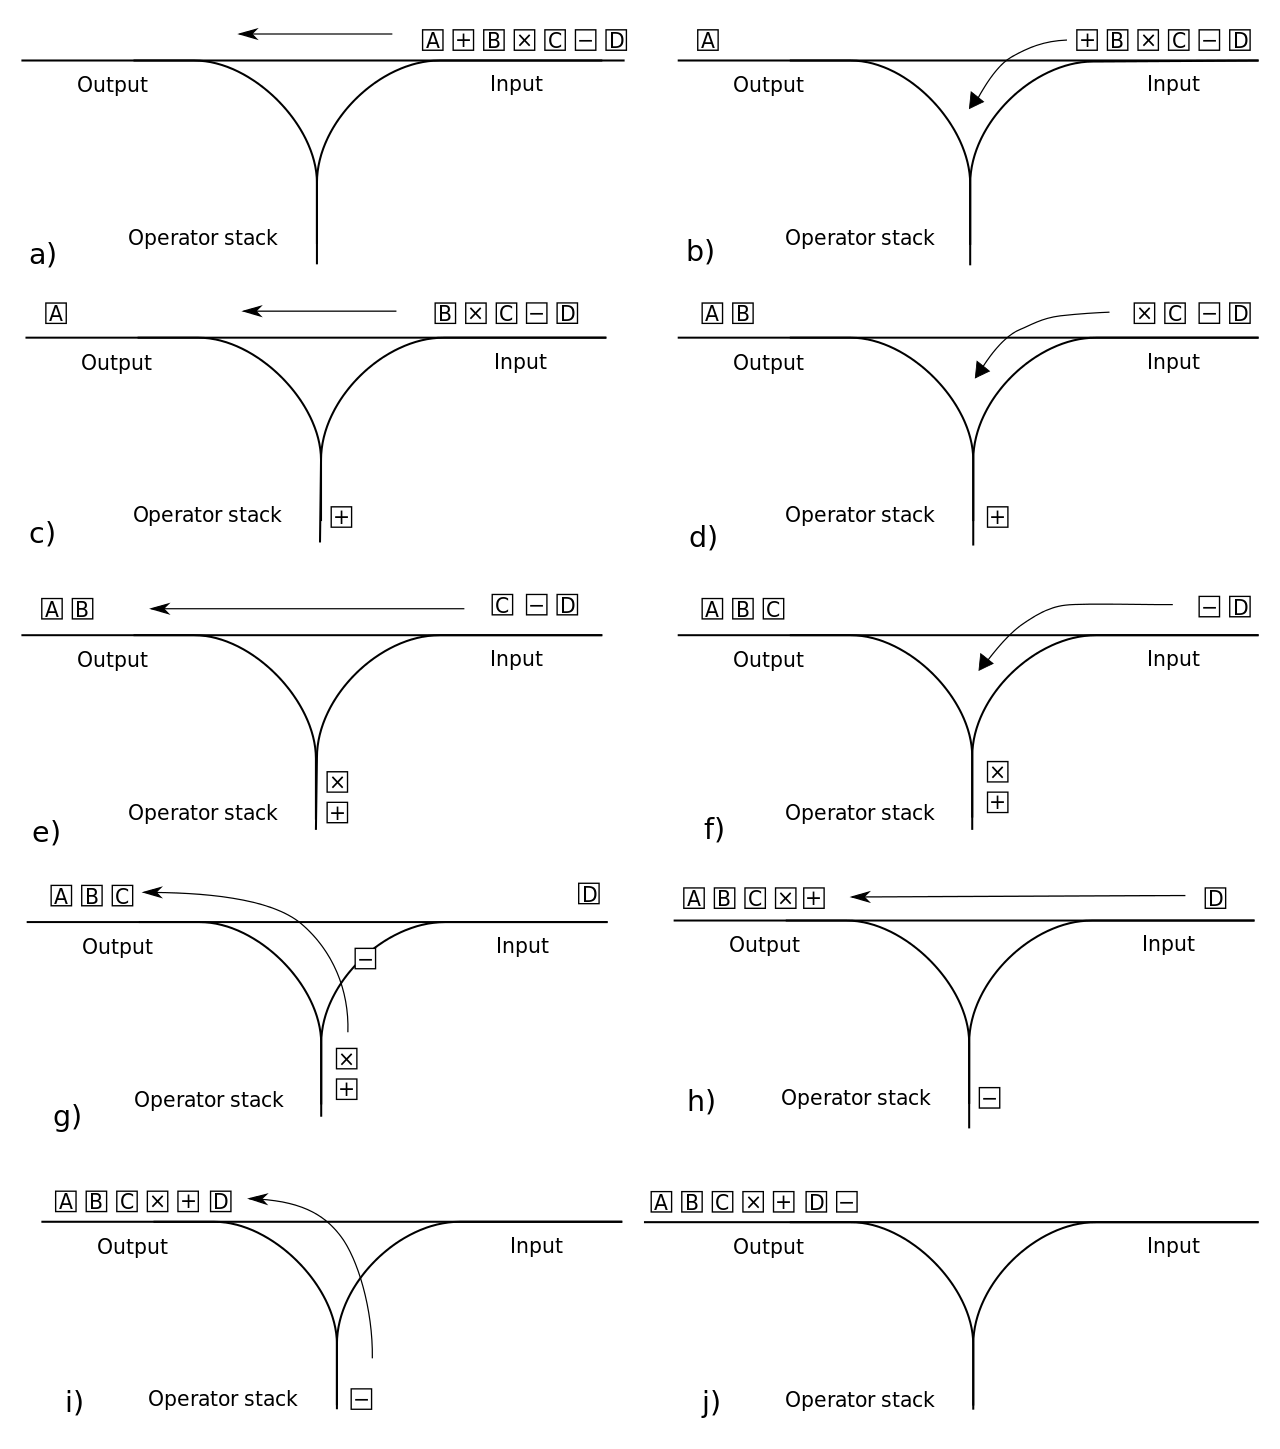
\includegraphics[width=5cm]{images/shunting_yard}
    \caption{Алгоритъм Shunting Yard. Източник: \href{https://en.wikipedia.org/wiki/Shunting-yard_algorithm}{Wikipedia}}
    \label{fig:syard}
    \end{figure}  
\end{frame}
  

\begin{frame}[fragile]
  \frametitle{Shunting Yard}
  \begin{itemize}
    \item Число: директно отива в изхода
    \item Оператор: изважда от върха на стека всички оператори с по-голям или равен приоритет
    \item Отваряща скоба: застава на върха на стека
    \item Затваряща скоба: изважда от стека всичко до отварящата скоба, като маха и нея
  \end{itemize}
\end{frame}


\begin{frame}
\centerline{Благодаря за вниманието!}
\end{frame}


\end{document}
 
\begin{columns}[t]
  \begin{column}{0.55\textwidth}

  \end{column}
  \begin{column}{0.45\textwidth}

  \end{column}
\end{columns}


